\documentclass[twoside]{book}

% Packages required by doxygen
\usepackage{fixltx2e}
\usepackage{calc}
\usepackage{doxygen}
\usepackage[export]{adjustbox} % also loads graphicx
\usepackage{graphicx}
\usepackage[utf8]{inputenc}
\usepackage{makeidx}
\usepackage{multicol}
\usepackage{multirow}
\PassOptionsToPackage{warn}{textcomp}
\usepackage{textcomp}
\usepackage[nointegrals]{wasysym}
\usepackage[table]{xcolor}

% Font selection
\usepackage[T1]{fontenc}
\usepackage[scaled=.90]{helvet}
\usepackage{courier}
\usepackage{amssymb}
\usepackage{sectsty}
\renewcommand{\familydefault}{\sfdefault}
\allsectionsfont{%
  \fontseries{bc}\selectfont%
  \color{darkgray}%
}
\renewcommand{\DoxyLabelFont}{%
  \fontseries{bc}\selectfont%
  \color{darkgray}%
}
\newcommand{\+}{\discretionary{\mbox{\scriptsize$\hookleftarrow$}}{}{}}

% Page & text layout
\usepackage{geometry}
\geometry{%
  a4paper,%
  top=2.5cm,%
  bottom=2.5cm,%
  left=2.5cm,%
  right=2.5cm%
}
\tolerance=750
\hfuzz=15pt
\hbadness=750
\setlength{\emergencystretch}{15pt}
\setlength{\parindent}{0cm}
\setlength{\parskip}{3ex plus 2ex minus 2ex}
\makeatletter
\renewcommand{\paragraph}{%
  \@startsection{paragraph}{4}{0ex}{-1.0ex}{1.0ex}{%
    \normalfont\normalsize\bfseries\SS@parafont%
  }%
}
\renewcommand{\subparagraph}{%
  \@startsection{subparagraph}{5}{0ex}{-1.0ex}{1.0ex}{%
    \normalfont\normalsize\bfseries\SS@subparafont%
  }%
}
\makeatother

% Headers & footers
\usepackage{fancyhdr}
\pagestyle{fancyplain}
\fancyhead[LE]{\fancyplain{}{\bfseries\thepage}}
\fancyhead[CE]{\fancyplain{}{}}
\fancyhead[RE]{\fancyplain{}{\bfseries\leftmark}}
\fancyhead[LO]{\fancyplain{}{\bfseries\rightmark}}
\fancyhead[CO]{\fancyplain{}{}}
\fancyhead[RO]{\fancyplain{}{\bfseries\thepage}}
\fancyfoot[LE]{\fancyplain{}{}}
\fancyfoot[CE]{\fancyplain{}{}}
\fancyfoot[RE]{\fancyplain{}{\bfseries\scriptsize Generated by Doxygen }}
\fancyfoot[LO]{\fancyplain{}{\bfseries\scriptsize Generated by Doxygen }}
\fancyfoot[CO]{\fancyplain{}{}}
\fancyfoot[RO]{\fancyplain{}{}}
\renewcommand{\footrulewidth}{0.4pt}
\renewcommand{\chaptermark}[1]{%
  \markboth{#1}{}%
}
\renewcommand{\sectionmark}[1]{%
  \markright{\thesection\ #1}%
}

% Indices & bibliography
\usepackage{natbib}
\usepackage[titles]{tocloft}
\setcounter{tocdepth}{3}
\setcounter{secnumdepth}{5}
\makeindex

% Hyperlinks (required, but should be loaded last)
\usepackage{ifpdf}
\ifpdf
  \usepackage[pdftex,pagebackref=true]{hyperref}
\else
  \usepackage[ps2pdf,pagebackref=true]{hyperref}
\fi
\hypersetup{%
  colorlinks=true,%
  linkcolor=blue,%
  citecolor=blue,%
  unicode%
}

% Custom commands
\newcommand{\clearemptydoublepage}{%
  \newpage{\pagestyle{empty}\cleardoublepage}%
}

\usepackage{caption}
\captionsetup{labelsep=space,justification=centering,font={bf},singlelinecheck=off,skip=4pt,position=top}

%===== C O N T E N T S =====

\begin{document}

% Titlepage & ToC
\hypersetup{pageanchor=false,
             bookmarksnumbered=true,
             pdfencoding=unicode
            }
\pagenumbering{alph}
\begin{titlepage}
\vspace*{7cm}
\begin{center}%
{\Large My Project }\\
\vspace*{1cm}
{\large Generated by Doxygen 1.8.14}\\
\end{center}
\end{titlepage}
\clearemptydoublepage
\pagenumbering{roman}
\tableofcontents
\clearemptydoublepage
\pagenumbering{arabic}
\hypersetup{pageanchor=true}

%--- Begin generated contents ---
\chapter{Namespace Index}
\section{Packages}
Here are the packages with brief descriptions (if available)\+:\begin{DoxyCompactList}
\item\contentsline{section}{\mbox{\hyperlink{namespace_super_mario}{Super\+Mario}} }{\pageref{namespace_super_mario}}{}
\item\contentsline{section}{\mbox{\hyperlink{namespace_super_mario_1_1_graphics}{Super\+Mario.\+Graphics}} }{\pageref{namespace_super_mario_1_1_graphics}}{}
\item\contentsline{section}{\mbox{\hyperlink{namespace_super_mario_1_1_level_components}{Super\+Mario.\+Level\+Components}} }{\pageref{namespace_super_mario_1_1_level_components}}{}
\end{DoxyCompactList}

\chapter{Hierarchical Index}
\section{Class Hierarchy}
This inheritance list is sorted roughly, but not completely, alphabetically\+:\begin{DoxyCompactList}
\item \contentsline{section}{Super\+Mario.\+Graphics.\+Animated\+Sprite}{\pageref{class_super_mario_1_1_graphics_1_1_animated_sprite}}{}
\item \contentsline{section}{Super\+Mario.\+Level\+Components.\+Block}{\pageref{class_super_mario_1_1_level_components_1_1_block}}{}
\begin{DoxyCompactList}
\item \contentsline{section}{Super\+Mario.\+Level\+Components.\+Dirt}{\pageref{class_super_mario_1_1_level_components_1_1_dirt}}{}
\end{DoxyCompactList}
\item \contentsline{section}{Super\+Mario.\+Camera}{\pageref{class_super_mario_1_1_camera}}{}
\item Game\begin{DoxyCompactList}
\item \contentsline{section}{Super\+Mario.\+Super\+Mario}{\pageref{class_super_mario_1_1_super_mario}}{}
\end{DoxyCompactList}
\item I\+Dictionary\begin{DoxyCompactList}
\item \contentsline{section}{Super\+Mario.\+Graphics.\+Animated\+Sprite\+Dictionary}{\pageref{class_super_mario_1_1_graphics_1_1_animated_sprite_dictionary}}{}
\begin{DoxyCompactList}
\item \contentsline{section}{Super\+Mario.\+Graphics.\+Mario\+Small\+Sprite\+Dictionary}{\pageref{class_super_mario_1_1_graphics_1_1_mario_small_sprite_dictionary}}{}
\end{DoxyCompactList}
\end{DoxyCompactList}
\item I\+Enumerable$<$ Key\+Value\+Pair$<$ Sprite\+Actions, Animated\+Sprite $>$$>$\begin{DoxyCompactList}
\item \contentsline{section}{Super\+Mario.\+Graphics.\+Animated\+Sprite\+Dictionary}{\pageref{class_super_mario_1_1_graphics_1_1_animated_sprite_dictionary}}{}
\end{DoxyCompactList}
\item \contentsline{section}{Super\+Mario.\+Level}{\pageref{class_super_mario_1_1_level}}{}
\item \contentsline{section}{Super\+Mario.\+Tile}{\pageref{class_super_mario_1_1_tile}}{}
\item \contentsline{section}{Super\+Mario.\+Level\+Components.\+Wall}{\pageref{class_super_mario_1_1_level_components_1_1_wall}}{}
\end{DoxyCompactList}

\chapter{Class Index}
\section{Class List}
Here are the classes, structs, unions and interfaces with brief descriptions\+:\begin{DoxyCompactList}
\item\contentsline{section}{\mbox{\hyperlink{class_super_mario_1_1_graphics_1_1_animated_sprite}{Super\+Mario.\+Graphics.\+Animated\+Sprite}} }{\pageref{class_super_mario_1_1_graphics_1_1_animated_sprite}}{}
\item\contentsline{section}{\mbox{\hyperlink{class_super_mario_1_1_graphics_1_1_animated_sprite_dictionary}{Super\+Mario.\+Graphics.\+Animated\+Sprite\+Dictionary}} }{\pageref{class_super_mario_1_1_graphics_1_1_animated_sprite_dictionary}}{}
\item\contentsline{section}{\mbox{\hyperlink{class_super_mario_1_1_level_components_1_1_block}{Super\+Mario.\+Level\+Components.\+Block}} \\*This class contains all the data for foreground \mbox{\hyperlink{class_super_mario_1_1_tile}{Tile}} objects }{\pageref{class_super_mario_1_1_level_components_1_1_block}}{}
\item\contentsline{section}{\mbox{\hyperlink{class_super_mario_1_1_camera}{Super\+Mario.\+Camera}} \\*Manages everything camera related }{\pageref{class_super_mario_1_1_camera}}{}
\item\contentsline{section}{\mbox{\hyperlink{class_super_mario_1_1_level_components_1_1_dirt}{Super\+Mario.\+Level\+Components.\+Dirt}} }{\pageref{class_super_mario_1_1_level_components_1_1_dirt}}{}
\item\contentsline{section}{\mbox{\hyperlink{class_super_mario_1_1_level}{Super\+Mario.\+Level}} }{\pageref{class_super_mario_1_1_level}}{}
\item\contentsline{section}{\mbox{\hyperlink{class_super_mario_1_1_graphics_1_1_mario_small_sprite_dictionary}{Super\+Mario.\+Graphics.\+Mario\+Small\+Sprite\+Dictionary}} }{\pageref{class_super_mario_1_1_graphics_1_1_mario_small_sprite_dictionary}}{}
\item\contentsline{section}{\mbox{\hyperlink{class_super_mario_1_1_super_mario}{Super\+Mario.\+Super\+Mario}} \\*This is the main type for your game. }{\pageref{class_super_mario_1_1_super_mario}}{}
\item\contentsline{section}{\mbox{\hyperlink{class_super_mario_1_1_tile}{Super\+Mario.\+Tile}} \\*Class that store infos about a particular tile }{\pageref{class_super_mario_1_1_tile}}{}
\item\contentsline{section}{\mbox{\hyperlink{class_super_mario_1_1_level_components_1_1_wall}{Super\+Mario.\+Level\+Components.\+Wall}} \\*This class contains all the data for background objects }{\pageref{class_super_mario_1_1_level_components_1_1_wall}}{}
\end{DoxyCompactList}

\chapter{Namespace Documentation}
\hypertarget{namespace_super_mario}{}\section{Super\+Mario Namespace Reference}
\label{namespace_super_mario}\index{Super\+Mario@{Super\+Mario}}
\subsection*{Namespaces}
\begin{DoxyCompactItemize}
\end{DoxyCompactItemize}
\subsection*{Classes}
\begin{DoxyCompactItemize}
\item 
class \mbox{\hyperlink{class_super_mario_1_1_camera}{Camera}}
\begin{DoxyCompactList}\small\item\em Manages everything camera related \end{DoxyCompactList}\item 
class {\bfseries Entity\+Id}
\begin{DoxyCompactList}\small\item\em Helper class that stores every object\textquotesingle{}s Id \end{DoxyCompactList}\item 
class \mbox{\hyperlink{class_super_mario_1_1_level}{Level}}
\item 
class \mbox{\hyperlink{class_super_mario_1_1_super_mario}{Super\+Mario}}
\begin{DoxyCompactList}\small\item\em This is the main type for your game. \end{DoxyCompactList}\item 
class \mbox{\hyperlink{class_super_mario_1_1_tile}{Tile}}
\begin{DoxyCompactList}\small\item\em Class that store infos about a particular tile \end{DoxyCompactList}\end{DoxyCompactItemize}

\hypertarget{namespace_super_mario_1_1_graphics}{}\section{Super\+Mario.\+Graphics Namespace Reference}
\label{namespace_super_mario_1_1_graphics}\index{Super\+Mario.\+Graphics@{Super\+Mario.\+Graphics}}
\subsection*{Classes}
\begin{DoxyCompactItemize}
\item 
class \mbox{\hyperlink{class_super_mario_1_1_graphics_1_1_animated_sprite}{Animated\+Sprite}}
\item 
class \mbox{\hyperlink{class_super_mario_1_1_graphics_1_1_animated_sprite_dictionary}{Animated\+Sprite\+Dictionary}}
\item 
class \mbox{\hyperlink{class_super_mario_1_1_graphics_1_1_mario_small_sprite_dictionary}{Mario\+Small\+Sprite\+Dictionary}}
\end{DoxyCompactItemize}
\subsection*{Enumerations}
\begin{DoxyCompactItemize}
\item 
\mbox{\Hypertarget{namespace_super_mario_1_1_graphics_ae4f4372bb75546bd6055162321094766}\label{namespace_super_mario_1_1_graphics_ae4f4372bb75546bd6055162321094766}} 
enum {\bfseries Sprite\+Actions} \{ \newline
{\bfseries Default}, 
{\bfseries Idle}, 
{\bfseries Walking}, 
{\bfseries Running}, 
\newline
{\bfseries Falling}, 
{\bfseries Croucing}
 \}
\end{DoxyCompactItemize}

\hypertarget{namespace_super_mario_1_1_level_components}{}\section{Super\+Mario.\+Level\+Components Namespace Reference}
\label{namespace_super_mario_1_1_level_components}\index{Super\+Mario.\+Level\+Components@{Super\+Mario.\+Level\+Components}}
\subsection*{Classes}
\begin{DoxyCompactItemize}
\item 
class \mbox{\hyperlink{class_super_mario_1_1_level_components_1_1_block}{Block}}
\begin{DoxyCompactList}\small\item\em This class contains all the data for foreground \mbox{\hyperlink{class_super_mario_1_1_tile}{Tile}} objects \end{DoxyCompactList}\item 
class \mbox{\hyperlink{class_super_mario_1_1_level_components_1_1_dirt}{Dirt}}
\item 
class \mbox{\hyperlink{class_super_mario_1_1_level_components_1_1_wall}{Wall}}
\begin{DoxyCompactList}\small\item\em This class contains all the data for background objects \end{DoxyCompactList}\end{DoxyCompactItemize}
\subsection*{Enumerations}
\begin{DoxyCompactItemize}
\item 
enum \mbox{\hyperlink{namespace_super_mario_1_1_level_components_a6fb13645a44790821090630fdf2b1afd}{Tile\+Mapping}} \{ \newline
{\bfseries Top\+Left\+Corner}, 
{\bfseries Top\+Middle\+Border}, 
{\bfseries Top\+Right\+Corner}, 
{\bfseries Bottom\+Right\+Inner\+Corner}, 
\newline
{\bfseries Bottom\+Left\+Inner\+Corner}, 
{\bfseries Top\+Left\+Corner\+Bottom\+Right\+Inner\+Corner}, 
{\bfseries Top\+Bottom\+Border}, 
{\bfseries Top\+Right\+Corner\+Bottom\+Left\+Inner\+Corner}, 
\newline
{\bfseries Left\+Border}, 
{\bfseries Center}, 
{\bfseries Right\+Border}, 
{\bfseries Top\+Right\+Inner\+Corner}, 
\newline
{\bfseries Top\+Left\+Inner\+Corner}, 
{\bfseries Left\+Right\+Border}, 
{\bfseries All\+Border}, 
{\bfseries Top\+Left\+Right\+Border}, 
\newline
{\bfseries Bottom\+Left\+Corner}, 
{\bfseries Bottom\+Middle\+Border}, 
{\bfseries Bottom\+Right\+Corner}, 
{\bfseries Top\+Left\+Bottom\+Border}, 
\newline
{\bfseries Top\+Right\+Bottom\+Border}, 
{\bfseries Bottom\+Left\+Corner\+Top\+Right\+Inner\+Corner}, 
{\bfseries Top\+Bottom\+Border2}, 
{\bfseries Bottom\+Right\+Corner\+Top\+Left\+Inner\+Corner}, 
\newline
{\bfseries Top\+Middle\+Border\+Bottom\+Right\+Inner\+Corner}, 
{\bfseries Top\+Middle\+Border\+Bottom\+Left\+Inner\+Corner}, 
{\bfseries Left\+Middle\+Border\+Bottom\+Right\+Inner\+Corner}, 
{\bfseries Right\+Middle\+Border\+Bottom\+Left\+Inner\+Corner}, 
\newline
{\bfseries Top\+Middle\+Border\+Bottom\+Left\+Inner\+Corner\+Bottom\+Righ\+Inner\+Corner}, 
{\bfseries Bottom\+Left\+Inner\+Corner\+Bottom\+Right\+Inner\+Corner}, 
{\bfseries Left\+Middle\+Border\+Top\+Right\+Inner\+Corner\+Bottom\+Right\+Inner\+Corner}, 
{\bfseries Right\+Middle\+Border\+Top\+Left\+Inner\+Corner\+Bottom\+Left\+Inner\+Corner}, 
\newline
{\bfseries Bottom\+Middle\+Border\+Top\+Right\+Inner\+Corner}, 
{\bfseries Bottom\+Middle\+Border\+Top\+Left\+Inner\+Corner}, 
{\bfseries Left\+Middle\+Border\+Top\+Right\+Inner\+Corner}, 
{\bfseries Right\+Middle\+Border\+Top\+Left\+Inner\+Corner}, 
\newline
{\bfseries Bottom\+Middle\+Border\+Top\+Left\+Inner\+Corner\+Top\+Right\+Inner\+Corner}, 
{\bfseries Top\+Left\+Inner\+Corner\+Top\+Right\+Inner\+Corner}, 
{\bfseries Top\+Right\+Inner\+Corner\+Bottom\+Right\+Inner\+Corner}, 
{\bfseries Top\+Left\+Inner\+Corner\+Bottom\+Left\+Inner\+Corner}, 
\newline
{\bfseries Top\+Left\+Inner\+Corner\+Top\+Right\+Inner\+Corner\+Bottom\+Left\+Inner\+Corner}, 
{\bfseries Top\+Left\+Inner\+Corner\+Top\+Right\+Inner\+Corner\+Bottom\+Right\+Inner\+Corner}, 
{\bfseries Top\+Right\+Inner\+Corner\+Bottom\+Left\+Inner\+Corner\+Bottom\+Right\+Inner\+Corner}, 
{\bfseries Top\+Left\+Inner\+Corner\+Bottom\+Left\+Inner\+Corner\+Bottom\+Right\+Inner\+Corner}, 
\newline
{\bfseries All\+Four\+Inner\+Corner}, 
{\bfseries Top\+Right\+Inner\+Corner\+Bottom\+Left\+Inner\+Corner}, 
{\bfseries Top\+Left\+Inner\+Corner\+Bottom\+Right\+Inner\+Corner}, 
{\bfseries Bottom\+Left\+Right\+Border}
 \}
\begin{DoxyCompactList}\small\item\em This Enum is used to easily identify each tile from the tileset in a sorted way \end{DoxyCompactList}\end{DoxyCompactItemize}


\subsection{Enumeration Type Documentation}
\mbox{\Hypertarget{namespace_super_mario_1_1_level_components_a6fb13645a44790821090630fdf2b1afd}\label{namespace_super_mario_1_1_level_components_a6fb13645a44790821090630fdf2b1afd}} 
\index{Super\+Mario\+::\+Level\+Components@{Super\+Mario\+::\+Level\+Components}!Tile\+Mapping@{Tile\+Mapping}}
\index{Tile\+Mapping@{Tile\+Mapping}!Super\+Mario\+::\+Level\+Components@{Super\+Mario\+::\+Level\+Components}}
\subsubsection{\texorpdfstring{Tile\+Mapping}{TileMapping}}
{\footnotesize\ttfamily enum \mbox{\hyperlink{namespace_super_mario_1_1_level_components_a6fb13645a44790821090630fdf2b1afd}{Super\+Mario.\+Level\+Components.\+Tile\+Mapping}}\hspace{0.3cm}{\ttfamily [strong]}}



This Enum is used to easily identify each tile from the tileset in a sorted way 


\chapter{Class Documentation}
\hypertarget{class_super_mario_1_1_graphics_1_1_animated_sprite}{}\section{Super\+Mario.\+Graphics.\+Animated\+Sprite Class Reference}
\label{class_super_mario_1_1_graphics_1_1_animated_sprite}\index{Super\+Mario.\+Graphics.\+Animated\+Sprite@{Super\+Mario.\+Graphics.\+Animated\+Sprite}}
\subsection*{Public Member Functions}
\begin{DoxyCompactItemize}
\item 
\mbox{\Hypertarget{class_super_mario_1_1_graphics_1_1_animated_sprite_a6458b19f7c9fc171e5fca0b880d2e229}\label{class_super_mario_1_1_graphics_1_1_animated_sprite_a6458b19f7c9fc171e5fca0b880d2e229}} 
{\bfseries Animated\+Sprite} (Texture2D texture, int total\+Frames, int columns, int rows, params int\mbox{[}$\,$\mbox{]} action\+Frames)
\item 
\mbox{\Hypertarget{class_super_mario_1_1_graphics_1_1_animated_sprite_aa11f2da4ed82e78a2386ad3d07d262a3}\label{class_super_mario_1_1_graphics_1_1_animated_sprite_aa11f2da4ed82e78a2386ad3d07d262a3}} 
void {\bfseries Update} (Game\+Time game\+Time)
\item 
\mbox{\Hypertarget{class_super_mario_1_1_graphics_1_1_animated_sprite_ab647c3ee7530a04ad1ac057201e0e8ed}\label{class_super_mario_1_1_graphics_1_1_animated_sprite_ab647c3ee7530a04ad1ac057201e0e8ed}} 
void {\bfseries Draw} (Sprite\+Batch sprite\+Batch, Vector2 position)
\end{DoxyCompactItemize}
\subsection*{Properties}
\begin{DoxyCompactItemize}
\item 
\mbox{\Hypertarget{class_super_mario_1_1_graphics_1_1_animated_sprite_a5f2a524155622c381ed4ca2a4c9e6fe9}\label{class_super_mario_1_1_graphics_1_1_animated_sprite_a5f2a524155622c381ed4ca2a4c9e6fe9}} 
int {\bfseries Total\+Frames}\hspace{0.3cm}{\ttfamily  \mbox{[}get, set\mbox{]}}
\end{DoxyCompactItemize}


The documentation for this class was generated from the following file\+:\begin{DoxyCompactItemize}
\item 
Graphics/Animated\+Sprite.\+cs\end{DoxyCompactItemize}

\hypertarget{class_super_mario_1_1_graphics_1_1_animated_sprite_dictionary}{}\section{Super\+Mario.\+Graphics.\+Animated\+Sprite\+Dictionary Class Reference}
\label{class_super_mario_1_1_graphics_1_1_animated_sprite_dictionary}\index{Super\+Mario.\+Graphics.\+Animated\+Sprite\+Dictionary@{Super\+Mario.\+Graphics.\+Animated\+Sprite\+Dictionary}}
Inheritance diagram for Super\+Mario.\+Graphics.\+Animated\+Sprite\+Dictionary\+:\begin{figure}[H]
\begin{center}
\leavevmode
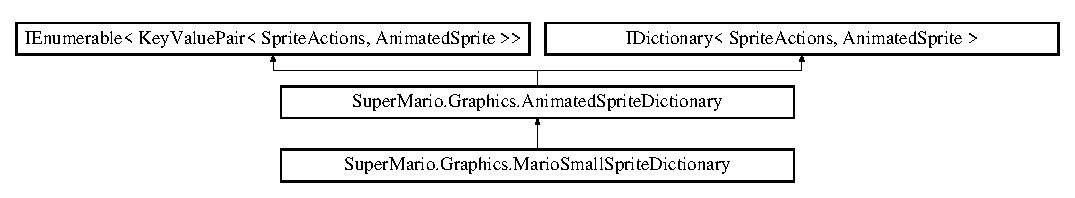
\includegraphics[height=2.210526cm]{class_super_mario_1_1_graphics_1_1_animated_sprite_dictionary}
\end{center}
\end{figure}
\subsection*{Public Member Functions}
\begin{DoxyCompactItemize}
\item 
\mbox{\Hypertarget{class_super_mario_1_1_graphics_1_1_animated_sprite_dictionary_a960f361d619281f48fb89304d2b53f25}\label{class_super_mario_1_1_graphics_1_1_animated_sprite_dictionary_a960f361d619281f48fb89304d2b53f25}} 
void {\bfseries Add} (Sprite\+Actions key, \mbox{\hyperlink{class_super_mario_1_1_graphics_1_1_animated_sprite}{Animated\+Sprite}} value)
\item 
\mbox{\Hypertarget{class_super_mario_1_1_graphics_1_1_animated_sprite_dictionary_ae62452172370e7431f4a66f2da863e88}\label{class_super_mario_1_1_graphics_1_1_animated_sprite_dictionary_ae62452172370e7431f4a66f2da863e88}} 
void {\bfseries Add} (Key\+Value\+Pair$<$ Sprite\+Actions, \mbox{\hyperlink{class_super_mario_1_1_graphics_1_1_animated_sprite}{Animated\+Sprite}} $>$ item)
\item 
\mbox{\Hypertarget{class_super_mario_1_1_graphics_1_1_animated_sprite_dictionary_aebf2c07421f4d13d85be04f3a1a93c8b}\label{class_super_mario_1_1_graphics_1_1_animated_sprite_dictionary_aebf2c07421f4d13d85be04f3a1a93c8b}} 
void {\bfseries Clear} ()
\item 
\mbox{\Hypertarget{class_super_mario_1_1_graphics_1_1_animated_sprite_dictionary_a42033bece722801e46cff223c542bc4f}\label{class_super_mario_1_1_graphics_1_1_animated_sprite_dictionary_a42033bece722801e46cff223c542bc4f}} 
bool {\bfseries Contains} (Key\+Value\+Pair$<$ Sprite\+Actions, \mbox{\hyperlink{class_super_mario_1_1_graphics_1_1_animated_sprite}{Animated\+Sprite}} $>$ item)
\item 
\mbox{\Hypertarget{class_super_mario_1_1_graphics_1_1_animated_sprite_dictionary_aeffcc0114d3e5a21e64ebb6bb9095fab}\label{class_super_mario_1_1_graphics_1_1_animated_sprite_dictionary_aeffcc0114d3e5a21e64ebb6bb9095fab}} 
bool {\bfseries Contains\+Key} (Sprite\+Actions key)
\item 
\mbox{\Hypertarget{class_super_mario_1_1_graphics_1_1_animated_sprite_dictionary_a8f3cacc1cffd58e8cd422abddba1c660}\label{class_super_mario_1_1_graphics_1_1_animated_sprite_dictionary_a8f3cacc1cffd58e8cd422abddba1c660}} 
void {\bfseries Copy\+To} (Key\+Value\+Pair$<$ Sprite\+Actions, \mbox{\hyperlink{class_super_mario_1_1_graphics_1_1_animated_sprite}{Animated\+Sprite}} $>$\mbox{[}$\,$\mbox{]} array, int array\+Index)
\item 
\mbox{\Hypertarget{class_super_mario_1_1_graphics_1_1_animated_sprite_dictionary_a8e92a31770d8f3eb62725b79af0dcf02}\label{class_super_mario_1_1_graphics_1_1_animated_sprite_dictionary_a8e92a31770d8f3eb62725b79af0dcf02}} 
I\+Enumerator$<$ Key\+Value\+Pair$<$ Sprite\+Actions, \mbox{\hyperlink{class_super_mario_1_1_graphics_1_1_animated_sprite}{Animated\+Sprite}} $>$ $>$ {\bfseries Get\+Enumerator} ()
\item 
\mbox{\Hypertarget{class_super_mario_1_1_graphics_1_1_animated_sprite_dictionary_a418ccd9832b2ecf1e701c45c6fd88333}\label{class_super_mario_1_1_graphics_1_1_animated_sprite_dictionary_a418ccd9832b2ecf1e701c45c6fd88333}} 
bool {\bfseries Remove} (Sprite\+Actions key)
\item 
\mbox{\Hypertarget{class_super_mario_1_1_graphics_1_1_animated_sprite_dictionary_af1a76ba4963173f9a69a708621f62cf4}\label{class_super_mario_1_1_graphics_1_1_animated_sprite_dictionary_af1a76ba4963173f9a69a708621f62cf4}} 
bool {\bfseries Remove} (Key\+Value\+Pair$<$ Sprite\+Actions, \mbox{\hyperlink{class_super_mario_1_1_graphics_1_1_animated_sprite}{Animated\+Sprite}} $>$ item)
\item 
\mbox{\Hypertarget{class_super_mario_1_1_graphics_1_1_animated_sprite_dictionary_a4e8e81af53ff5050bca7bededde39fda}\label{class_super_mario_1_1_graphics_1_1_animated_sprite_dictionary_a4e8e81af53ff5050bca7bededde39fda}} 
bool {\bfseries Try\+Get\+Value} (Sprite\+Actions key, out \mbox{\hyperlink{class_super_mario_1_1_graphics_1_1_animated_sprite}{Animated\+Sprite}} value)
\end{DoxyCompactItemize}
\subsection*{Public Attributes}
\begin{DoxyCompactItemize}
\item 
\mbox{\Hypertarget{class_super_mario_1_1_graphics_1_1_animated_sprite_dictionary_a0bf6bcab7f15fe0c3a4f977a5c5d9d0d}\label{class_super_mario_1_1_graphics_1_1_animated_sprite_dictionary_a0bf6bcab7f15fe0c3a4f977a5c5d9d0d}} 
I\+Collection$<$ Sprite\+Actions $>$ {\bfseries Keys} =$>$ animated\+Sprites.\+Keys
\item 
\mbox{\Hypertarget{class_super_mario_1_1_graphics_1_1_animated_sprite_dictionary_aaf91ddcf162555516aef5fe5b71e7551}\label{class_super_mario_1_1_graphics_1_1_animated_sprite_dictionary_aaf91ddcf162555516aef5fe5b71e7551}} 
I\+Collection$<$ \mbox{\hyperlink{class_super_mario_1_1_graphics_1_1_animated_sprite}{Animated\+Sprite}} $>$ {\bfseries Values} =$>$ animated\+Sprites.\+Values
\item 
\mbox{\Hypertarget{class_super_mario_1_1_graphics_1_1_animated_sprite_dictionary_a2f4220f8c46030c4d674be2feabcb954}\label{class_super_mario_1_1_graphics_1_1_animated_sprite_dictionary_a2f4220f8c46030c4d674be2feabcb954}} 
int {\bfseries Count} =$>$ animated\+Sprites.\+Count
\item 
\mbox{\Hypertarget{class_super_mario_1_1_graphics_1_1_animated_sprite_dictionary_a8082d7ae6cf8e4df5bbe4be9816e2624}\label{class_super_mario_1_1_graphics_1_1_animated_sprite_dictionary_a8082d7ae6cf8e4df5bbe4be9816e2624}} 
bool {\bfseries Is\+Read\+Only} =$>$ false
\end{DoxyCompactItemize}
\subsection*{Protected Member Functions}
\begin{DoxyCompactItemize}
\item 
\mbox{\Hypertarget{class_super_mario_1_1_graphics_1_1_animated_sprite_dictionary_ac413d262ece4b3e18b18691096ac81fe}\label{class_super_mario_1_1_graphics_1_1_animated_sprite_dictionary_ac413d262ece4b3e18b18691096ac81fe}} 
abstract void {\bfseries Add\+Animated\+Sprites} ()
\end{DoxyCompactItemize}
\subsection*{Properties}
\begin{DoxyCompactItemize}
\item 
\mbox{\Hypertarget{class_super_mario_1_1_graphics_1_1_animated_sprite_dictionary_a16d79f77d8d8d24da7733ffb2e364316}\label{class_super_mario_1_1_graphics_1_1_animated_sprite_dictionary_a16d79f77d8d8d24da7733ffb2e364316}} 
\mbox{\hyperlink{class_super_mario_1_1_graphics_1_1_animated_sprite}{Animated\+Sprite}} {\bfseries this\mbox{[}\+Sprite\+Actions key\mbox{]}}\hspace{0.3cm}{\ttfamily  \mbox{[}get, set\mbox{]}}
\end{DoxyCompactItemize}


The documentation for this class was generated from the following file\+:\begin{DoxyCompactItemize}
\item 
Graphics/Animated\+Sprite\+Collection.\+cs\end{DoxyCompactItemize}

\hypertarget{class_super_mario_1_1_level_components_1_1_block}{}\section{Super\+Mario.\+Level\+Components.\+Block Class Reference}
\label{class_super_mario_1_1_level_components_1_1_block}\index{Super\+Mario.\+Level\+Components.\+Block@{Super\+Mario.\+Level\+Components.\+Block}}


This class contains all the data for foreground \mbox{\hyperlink{class_super_mario_1_1_tile}{Tile}} objects  


Inheritance diagram for Super\+Mario.\+Level\+Components.\+Block\+:\begin{figure}[H]
\begin{center}
\leavevmode
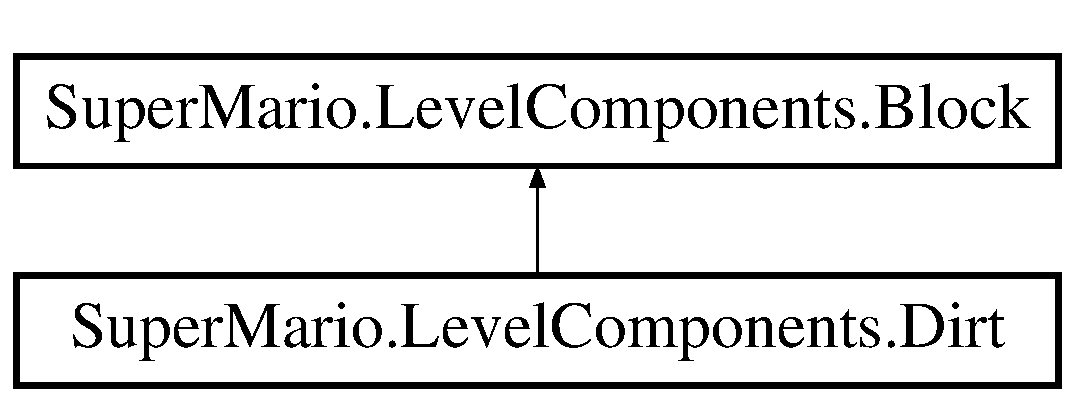
\includegraphics[height=2.000000cm]{class_super_mario_1_1_level_components_1_1_block}
\end{center}
\end{figure}
\subsection*{Public Member Functions}
\begin{DoxyCompactItemize}
\item 
abstract void \mbox{\hyperlink{class_super_mario_1_1_level_components_1_1_block_aecd2a6fa80ecbd7dd5cec2cdf4b149ec}{On\+Initialize}} ()
\begin{DoxyCompactList}\small\item\em This method is used to specify particular properties of the block (e.\+g. Id, Solid...) \end{DoxyCompactList}\end{DoxyCompactItemize}
\subsection*{Static Public Member Functions}
\begin{DoxyCompactItemize}
\item 
static Rectangle \mbox{\hyperlink{class_super_mario_1_1_level_components_1_1_block_afe826a9b23099b58f623e19b0422a3c0}{Get\+Frame}} (\mbox{\hyperlink{namespace_super_mario_1_1_level_components_a6fb13645a44790821090630fdf2b1afd}{Tile\+Mapping}} frame)
\begin{DoxyCompactList}\small\item\em Each tile set is made of a 8x6 grid and between each frame \end{DoxyCompactList}\item 
static Rectangle \mbox{\hyperlink{class_super_mario_1_1_level_components_1_1_block_a507402c0bd93c4659b28144580460ab9}{Get\+Frame}} (int x, int y, int tile\+Id)
\begin{DoxyCompactList}\small\item\em Calculate the correct frame to display on screen from the tileset \end{DoxyCompactList}\item 
static byte \mbox{\hyperlink{class_super_mario_1_1_level_components_1_1_block_a127645fecf73dad73e2e94d8e31ee11c}{Get\+Bit\+Mapping}} (int x, int y, int tile\+Id)
\begin{DoxyCompactList}\small\item\em Calculates the bit-\/mapping for the tileset to choose the correct frame refer to this

for more infos \end{DoxyCompactList}\item 
static \mbox{\hyperlink{namespace_super_mario_1_1_level_components_a6fb13645a44790821090630fdf2b1afd}{Tile\+Mapping}} \mbox{\hyperlink{class_super_mario_1_1_level_components_1_1_block_a58d5fb03dafc9daf7462446e16f666d7}{Get\+Tile\+From\+Bit}} (byte value)
\begin{DoxyCompactList}\small\item\em Returns the correct \mbox{\hyperlink{namespace_super_mario_1_1_level_components_a6fb13645a44790821090630fdf2b1afd}{Tile\+Mapping}} element from a Bit\+Map input value \end{DoxyCompactList}\end{DoxyCompactItemize}
\subsection*{Public Attributes}
\begin{DoxyCompactItemize}
\item 
const int \mbox{\hyperlink{class_super_mario_1_1_level_components_1_1_block_a43713182fbfda3b03101f02efb1d7fab}{C\+O\+L\+U\+M\+NS}} = 8
\begin{DoxyCompactList}\small\item\em The tileset\textquotesingle{}s number of frame per row \end{DoxyCompactList}\item 
const int \mbox{\hyperlink{class_super_mario_1_1_level_components_1_1_block_a28664c83dbf40588e8d769d440969f7c}{R\+O\+WS}} = 6
\begin{DoxyCompactList}\small\item\em The number of frames per column \end{DoxyCompactList}\item 
const int \mbox{\hyperlink{class_super_mario_1_1_level_components_1_1_block_a8a30649060abf7009666ac200da97d2e}{T\+I\+L\+E\+\_\+\+S\+I\+ZE}} = 16
\begin{DoxyCompactList}\small\item\em Standard size of a single frame \end{DoxyCompactList}\item 
const int \mbox{\hyperlink{class_super_mario_1_1_level_components_1_1_block_af3e47b544c2acb1f5cb0e3089ae7b774}{T\+I\+L\+E\+\_\+\+P\+A\+D\+D\+I\+NG}} = 1
\begin{DoxyCompactList}\small\item\em Padding between each frame in the tileset \end{DoxyCompactList}\item 
readonly Texture2D \mbox{\hyperlink{class_super_mario_1_1_level_components_1_1_block_a5176b65c486155dea95ef69ef94e16f4}{Tile\+Set}}
\begin{DoxyCompactList}\small\item\em The actual Texture\+Atlas \end{DoxyCompactList}\end{DoxyCompactItemize}
\subsection*{Protected Member Functions}
\begin{DoxyCompactItemize}
\item 
\mbox{\hyperlink{class_super_mario_1_1_level_components_1_1_block_a0a4ef8a1af9e91bd1e5774c90e74e65d}{Block}} ()
\begin{DoxyCompactList}\small\item\em Initializes the custom properties from \mbox{\hyperlink{class_super_mario_1_1_level_components_1_1_block_aecd2a6fa80ecbd7dd5cec2cdf4b149ec}{On\+Initialize}} and loads the tileset from \char`\"{}\+Blocks/\+Class\+Name\char`\"{} path in content pipeline \end{DoxyCompactList}\end{DoxyCompactItemize}
\subsection*{Properties}
\begin{DoxyCompactItemize}
\item 
int \mbox{\hyperlink{class_super_mario_1_1_level_components_1_1_block_ac3af8077575bf6621dc81d8566857af5}{Id}}\hspace{0.3cm}{\ttfamily  \mbox{[}get, protected set\mbox{]}}
\begin{DoxyCompactList}\small\item\em The Id used to identify this block, used in \mbox{\hyperlink{class_super_mario_1_1_tile}{Tile}} \end{DoxyCompactList}\end{DoxyCompactItemize}


\subsection{Detailed Description}
This class contains all the data for foreground \mbox{\hyperlink{class_super_mario_1_1_tile}{Tile}} objects 



\subsection{Constructor \& Destructor Documentation}
\mbox{\Hypertarget{class_super_mario_1_1_level_components_1_1_block_a0a4ef8a1af9e91bd1e5774c90e74e65d}\label{class_super_mario_1_1_level_components_1_1_block_a0a4ef8a1af9e91bd1e5774c90e74e65d}} 
\index{Super\+Mario\+::\+Level\+Components\+::\+Block@{Super\+Mario\+::\+Level\+Components\+::\+Block}!Block@{Block}}
\index{Block@{Block}!Super\+Mario\+::\+Level\+Components\+::\+Block@{Super\+Mario\+::\+Level\+Components\+::\+Block}}
\subsubsection{\texorpdfstring{Block()}{Block()}}
{\footnotesize\ttfamily Super\+Mario.\+Level\+Components.\+Block.\+Block (\begin{DoxyParamCaption}{ }\end{DoxyParamCaption})\hspace{0.3cm}{\ttfamily [protected]}}



Initializes the custom properties from \mbox{\hyperlink{class_super_mario_1_1_level_components_1_1_block_aecd2a6fa80ecbd7dd5cec2cdf4b149ec}{On\+Initialize}} and loads the tileset from \char`\"{}\+Blocks/\+Class\+Name\char`\"{} path in content pipeline 



\subsection{Member Function Documentation}
\mbox{\Hypertarget{class_super_mario_1_1_level_components_1_1_block_a127645fecf73dad73e2e94d8e31ee11c}\label{class_super_mario_1_1_level_components_1_1_block_a127645fecf73dad73e2e94d8e31ee11c}} 
\index{Super\+Mario\+::\+Level\+Components\+::\+Block@{Super\+Mario\+::\+Level\+Components\+::\+Block}!Get\+Bit\+Mapping@{Get\+Bit\+Mapping}}
\index{Get\+Bit\+Mapping@{Get\+Bit\+Mapping}!Super\+Mario\+::\+Level\+Components\+::\+Block@{Super\+Mario\+::\+Level\+Components\+::\+Block}}
\subsubsection{\texorpdfstring{Get\+Bit\+Mapping()}{GetBitMapping()}}
{\footnotesize\ttfamily static byte Super\+Mario.\+Level\+Components.\+Block.\+Get\+Bit\+Mapping (\begin{DoxyParamCaption}\item[{int}]{x,  }\item[{int}]{y,  }\item[{int}]{tile\+Id }\end{DoxyParamCaption})\hspace{0.3cm}{\ttfamily [static]}}



Calculates the bit-\/mapping for the tileset to choose the correct frame refer to this

for more infos 


\begin{DoxyParams}{Parameters}
{\em x} & x-\/coord of the tile in Super\+Mario.\+Main.\+tiles\\
\hline
{\em y} & y-\/coord of the tile in Super\+Mario.\+Main.\+tiles array\\
\hline
{\em tile\+Id} & the tile\textquotesingle{}s id to check against\\
\hline
\end{DoxyParams}
\begin{DoxyReturn}{Returns}
The bitmap value to be used in Get\+Tile\+From\+Bit method
\end{DoxyReturn}
\mbox{\Hypertarget{class_super_mario_1_1_level_components_1_1_block_afe826a9b23099b58f623e19b0422a3c0}\label{class_super_mario_1_1_level_components_1_1_block_afe826a9b23099b58f623e19b0422a3c0}} 
\index{Super\+Mario\+::\+Level\+Components\+::\+Block@{Super\+Mario\+::\+Level\+Components\+::\+Block}!Get\+Frame@{Get\+Frame}}
\index{Get\+Frame@{Get\+Frame}!Super\+Mario\+::\+Level\+Components\+::\+Block@{Super\+Mario\+::\+Level\+Components\+::\+Block}}
\subsubsection{\texorpdfstring{Get\+Frame()}{GetFrame()}\hspace{0.1cm}{\footnotesize\ttfamily [1/2]}}
{\footnotesize\ttfamily static Rectangle Super\+Mario.\+Level\+Components.\+Block.\+Get\+Frame (\begin{DoxyParamCaption}\item[{\mbox{\hyperlink{namespace_super_mario_1_1_level_components_a6fb13645a44790821090630fdf2b1afd}{Tile\+Mapping}}}]{frame }\end{DoxyParamCaption})\hspace{0.3cm}{\ttfamily [static]}}



Each tile set is made of a 8x6 grid and between each frame 


\begin{DoxyParams}{Parameters}
{\em frame} & The particular frame to select (e.\+g. a corner or a border)\\
\hline
\end{DoxyParams}
\begin{DoxyReturn}{Returns}
The Rectangle coordinates on the tile\+Set
\end{DoxyReturn}
\mbox{\Hypertarget{class_super_mario_1_1_level_components_1_1_block_a507402c0bd93c4659b28144580460ab9}\label{class_super_mario_1_1_level_components_1_1_block_a507402c0bd93c4659b28144580460ab9}} 
\index{Super\+Mario\+::\+Level\+Components\+::\+Block@{Super\+Mario\+::\+Level\+Components\+::\+Block}!Get\+Frame@{Get\+Frame}}
\index{Get\+Frame@{Get\+Frame}!Super\+Mario\+::\+Level\+Components\+::\+Block@{Super\+Mario\+::\+Level\+Components\+::\+Block}}
\subsubsection{\texorpdfstring{Get\+Frame()}{GetFrame()}\hspace{0.1cm}{\footnotesize\ttfamily [2/2]}}
{\footnotesize\ttfamily static Rectangle Super\+Mario.\+Level\+Components.\+Block.\+Get\+Frame (\begin{DoxyParamCaption}\item[{int}]{x,  }\item[{int}]{y,  }\item[{int}]{tile\+Id }\end{DoxyParamCaption})\hspace{0.3cm}{\ttfamily [static]}}



Calculate the correct frame to display on screen from the tileset 


\begin{DoxyParams}{Parameters}
{\em x} & x-\/coord of the tile in Super\+Mario.\+Main.\+tiles\\
\hline
{\em y} & y-\/coord of the tile in Super\+Mario.\+Main.\+tiles array\\
\hline
{\em tile\+Id} & the tile\textquotesingle{}s id to check against\\
\hline
\end{DoxyParams}
\begin{DoxyReturn}{Returns}

\end{DoxyReturn}
\mbox{\Hypertarget{class_super_mario_1_1_level_components_1_1_block_a58d5fb03dafc9daf7462446e16f666d7}\label{class_super_mario_1_1_level_components_1_1_block_a58d5fb03dafc9daf7462446e16f666d7}} 
\index{Super\+Mario\+::\+Level\+Components\+::\+Block@{Super\+Mario\+::\+Level\+Components\+::\+Block}!Get\+Tile\+From\+Bit@{Get\+Tile\+From\+Bit}}
\index{Get\+Tile\+From\+Bit@{Get\+Tile\+From\+Bit}!Super\+Mario\+::\+Level\+Components\+::\+Block@{Super\+Mario\+::\+Level\+Components\+::\+Block}}
\subsubsection{\texorpdfstring{Get\+Tile\+From\+Bit()}{GetTileFromBit()}}
{\footnotesize\ttfamily static \mbox{\hyperlink{namespace_super_mario_1_1_level_components_a6fb13645a44790821090630fdf2b1afd}{Tile\+Mapping}} Super\+Mario.\+Level\+Components.\+Block.\+Get\+Tile\+From\+Bit (\begin{DoxyParamCaption}\item[{byte}]{value }\end{DoxyParamCaption})\hspace{0.3cm}{\ttfamily [static]}}



Returns the correct \mbox{\hyperlink{namespace_super_mario_1_1_level_components_a6fb13645a44790821090630fdf2b1afd}{Tile\+Mapping}} element from a Bit\+Map input value 


\begin{DoxyParams}{Parameters}
{\em value} & The Bit\+Map value resulted from \mbox{\hyperlink{class_super_mario_1_1_level_components_1_1_block_a127645fecf73dad73e2e94d8e31ee11c}{Get\+Bit\+Mapping(int, int, int)}}\\
\hline
\end{DoxyParams}
\begin{DoxyReturn}{Returns}

\end{DoxyReturn}
\mbox{\Hypertarget{class_super_mario_1_1_level_components_1_1_block_aecd2a6fa80ecbd7dd5cec2cdf4b149ec}\label{class_super_mario_1_1_level_components_1_1_block_aecd2a6fa80ecbd7dd5cec2cdf4b149ec}} 
\index{Super\+Mario\+::\+Level\+Components\+::\+Block@{Super\+Mario\+::\+Level\+Components\+::\+Block}!On\+Initialize@{On\+Initialize}}
\index{On\+Initialize@{On\+Initialize}!Super\+Mario\+::\+Level\+Components\+::\+Block@{Super\+Mario\+::\+Level\+Components\+::\+Block}}
\subsubsection{\texorpdfstring{On\+Initialize()}{OnInitialize()}}
{\footnotesize\ttfamily abstract void Super\+Mario.\+Level\+Components.\+Block.\+On\+Initialize (\begin{DoxyParamCaption}{ }\end{DoxyParamCaption})\hspace{0.3cm}{\ttfamily [pure virtual]}}



This method is used to specify particular properties of the block (e.\+g. Id, Solid...) 



Implemented in \mbox{\hyperlink{class_super_mario_1_1_level_components_1_1_dirt_a800acb34aa293bf29cd3e4af39020633}{Super\+Mario.\+Level\+Components.\+Dirt}}.



\subsection{Member Data Documentation}
\mbox{\Hypertarget{class_super_mario_1_1_level_components_1_1_block_a43713182fbfda3b03101f02efb1d7fab}\label{class_super_mario_1_1_level_components_1_1_block_a43713182fbfda3b03101f02efb1d7fab}} 
\index{Super\+Mario\+::\+Level\+Components\+::\+Block@{Super\+Mario\+::\+Level\+Components\+::\+Block}!C\+O\+L\+U\+M\+NS@{C\+O\+L\+U\+M\+NS}}
\index{C\+O\+L\+U\+M\+NS@{C\+O\+L\+U\+M\+NS}!Super\+Mario\+::\+Level\+Components\+::\+Block@{Super\+Mario\+::\+Level\+Components\+::\+Block}}
\subsubsection{\texorpdfstring{C\+O\+L\+U\+M\+NS}{COLUMNS}}
{\footnotesize\ttfamily const int Super\+Mario.\+Level\+Components.\+Block.\+C\+O\+L\+U\+M\+NS = 8}



The tileset\textquotesingle{}s number of frame per row 

\mbox{\Hypertarget{class_super_mario_1_1_level_components_1_1_block_a28664c83dbf40588e8d769d440969f7c}\label{class_super_mario_1_1_level_components_1_1_block_a28664c83dbf40588e8d769d440969f7c}} 
\index{Super\+Mario\+::\+Level\+Components\+::\+Block@{Super\+Mario\+::\+Level\+Components\+::\+Block}!R\+O\+WS@{R\+O\+WS}}
\index{R\+O\+WS@{R\+O\+WS}!Super\+Mario\+::\+Level\+Components\+::\+Block@{Super\+Mario\+::\+Level\+Components\+::\+Block}}
\subsubsection{\texorpdfstring{R\+O\+WS}{ROWS}}
{\footnotesize\ttfamily const int Super\+Mario.\+Level\+Components.\+Block.\+R\+O\+WS = 6}



The number of frames per column 

\mbox{\Hypertarget{class_super_mario_1_1_level_components_1_1_block_af3e47b544c2acb1f5cb0e3089ae7b774}\label{class_super_mario_1_1_level_components_1_1_block_af3e47b544c2acb1f5cb0e3089ae7b774}} 
\index{Super\+Mario\+::\+Level\+Components\+::\+Block@{Super\+Mario\+::\+Level\+Components\+::\+Block}!T\+I\+L\+E\+\_\+\+P\+A\+D\+D\+I\+NG@{T\+I\+L\+E\+\_\+\+P\+A\+D\+D\+I\+NG}}
\index{T\+I\+L\+E\+\_\+\+P\+A\+D\+D\+I\+NG@{T\+I\+L\+E\+\_\+\+P\+A\+D\+D\+I\+NG}!Super\+Mario\+::\+Level\+Components\+::\+Block@{Super\+Mario\+::\+Level\+Components\+::\+Block}}
\subsubsection{\texorpdfstring{T\+I\+L\+E\+\_\+\+P\+A\+D\+D\+I\+NG}{TILE\_PADDING}}
{\footnotesize\ttfamily const int Super\+Mario.\+Level\+Components.\+Block.\+T\+I\+L\+E\+\_\+\+P\+A\+D\+D\+I\+NG = 1}



Padding between each frame in the tileset 

T\+O\+DO\+: fully implement or scrap this feature \mbox{\Hypertarget{class_super_mario_1_1_level_components_1_1_block_a8a30649060abf7009666ac200da97d2e}\label{class_super_mario_1_1_level_components_1_1_block_a8a30649060abf7009666ac200da97d2e}} 
\index{Super\+Mario\+::\+Level\+Components\+::\+Block@{Super\+Mario\+::\+Level\+Components\+::\+Block}!T\+I\+L\+E\+\_\+\+S\+I\+ZE@{T\+I\+L\+E\+\_\+\+S\+I\+ZE}}
\index{T\+I\+L\+E\+\_\+\+S\+I\+ZE@{T\+I\+L\+E\+\_\+\+S\+I\+ZE}!Super\+Mario\+::\+Level\+Components\+::\+Block@{Super\+Mario\+::\+Level\+Components\+::\+Block}}
\subsubsection{\texorpdfstring{T\+I\+L\+E\+\_\+\+S\+I\+ZE}{TILE\_SIZE}}
{\footnotesize\ttfamily const int Super\+Mario.\+Level\+Components.\+Block.\+T\+I\+L\+E\+\_\+\+S\+I\+ZE = 16}



Standard size of a single frame 

\mbox{\Hypertarget{class_super_mario_1_1_level_components_1_1_block_a5176b65c486155dea95ef69ef94e16f4}\label{class_super_mario_1_1_level_components_1_1_block_a5176b65c486155dea95ef69ef94e16f4}} 
\index{Super\+Mario\+::\+Level\+Components\+::\+Block@{Super\+Mario\+::\+Level\+Components\+::\+Block}!Tile\+Set@{Tile\+Set}}
\index{Tile\+Set@{Tile\+Set}!Super\+Mario\+::\+Level\+Components\+::\+Block@{Super\+Mario\+::\+Level\+Components\+::\+Block}}
\subsubsection{\texorpdfstring{Tile\+Set}{TileSet}}
{\footnotesize\ttfamily readonly Texture2D Super\+Mario.\+Level\+Components.\+Block.\+Tile\+Set}



The actual Texture\+Atlas 



\subsection{Property Documentation}
\mbox{\Hypertarget{class_super_mario_1_1_level_components_1_1_block_ac3af8077575bf6621dc81d8566857af5}\label{class_super_mario_1_1_level_components_1_1_block_ac3af8077575bf6621dc81d8566857af5}} 
\index{Super\+Mario\+::\+Level\+Components\+::\+Block@{Super\+Mario\+::\+Level\+Components\+::\+Block}!Id@{Id}}
\index{Id@{Id}!Super\+Mario\+::\+Level\+Components\+::\+Block@{Super\+Mario\+::\+Level\+Components\+::\+Block}}
\subsubsection{\texorpdfstring{Id}{Id}}
{\footnotesize\ttfamily int Super\+Mario.\+Level\+Components.\+Block.\+Id\hspace{0.3cm}{\ttfamily [get]}, {\ttfamily [protected set]}}



The Id used to identify this block, used in \mbox{\hyperlink{class_super_mario_1_1_tile}{Tile}} 



The documentation for this class was generated from the following file\+:\begin{DoxyCompactItemize}
\item 
Level\+Components/Block.\+cs\end{DoxyCompactItemize}

\hypertarget{class_super_mario_1_1_camera}{}\section{Super\+Mario.\+Camera Class Reference}
\label{class_super_mario_1_1_camera}\index{Super\+Mario.\+Camera@{Super\+Mario.\+Camera}}


Manages everything camera related  


\subsection*{Public Member Functions}
\begin{DoxyCompactItemize}
\item 
\mbox{\hyperlink{class_super_mario_1_1_camera_a5828416f8cef0538d1fe07bb31bf5f69}{Camera}} ()
\begin{DoxyCompactList}\small\item\em Creates the \mbox{\hyperlink{class_super_mario_1_1_camera}{Camera}} with some default values \end{DoxyCompactList}\item 
void \mbox{\hyperlink{class_super_mario_1_1_camera_a0fb046d2afebef6dd9a6507505909ec3}{Update}} ()
\begin{DoxyCompactList}\small\item\em Updates the matrix used in the spritebatch function \end{DoxyCompactList}\end{DoxyCompactItemize}
\subsection*{Public Attributes}
\begin{DoxyCompactItemize}
\item 
Vector2 \mbox{\hyperlink{class_super_mario_1_1_camera_a7dad8a59e38607abdc8fc8110e91d8d5}{position}}
\begin{DoxyCompactList}\small\item\em Position of the camera on the level \end{DoxyCompactList}\end{DoxyCompactItemize}
\subsection*{Properties}
\begin{DoxyCompactItemize}
\item 
Matrix \mbox{\hyperlink{class_super_mario_1_1_camera_aa1e50a0b539ec3092518b2c37984bb05}{Matrix}}\hspace{0.3cm}{\ttfamily  \mbox{[}get, set\mbox{]}}
\begin{DoxyCompactList}\small\item\em Transformation matrix that can be used for particular effects \end{DoxyCompactList}\end{DoxyCompactItemize}


\subsection{Detailed Description}
Manages everything camera related 



\subsection{Constructor \& Destructor Documentation}
\mbox{\Hypertarget{class_super_mario_1_1_camera_a5828416f8cef0538d1fe07bb31bf5f69}\label{class_super_mario_1_1_camera_a5828416f8cef0538d1fe07bb31bf5f69}} 
\index{Super\+Mario\+::\+Camera@{Super\+Mario\+::\+Camera}!Camera@{Camera}}
\index{Camera@{Camera}!Super\+Mario\+::\+Camera@{Super\+Mario\+::\+Camera}}
\subsubsection{\texorpdfstring{Camera()}{Camera()}}
{\footnotesize\ttfamily Super\+Mario.\+Camera.\+Camera (\begin{DoxyParamCaption}{ }\end{DoxyParamCaption})}



Creates the \mbox{\hyperlink{class_super_mario_1_1_camera}{Camera}} with some default values 



\subsection{Member Function Documentation}
\mbox{\Hypertarget{class_super_mario_1_1_camera_a0fb046d2afebef6dd9a6507505909ec3}\label{class_super_mario_1_1_camera_a0fb046d2afebef6dd9a6507505909ec3}} 
\index{Super\+Mario\+::\+Camera@{Super\+Mario\+::\+Camera}!Update@{Update}}
\index{Update@{Update}!Super\+Mario\+::\+Camera@{Super\+Mario\+::\+Camera}}
\subsubsection{\texorpdfstring{Update()}{Update()}}
{\footnotesize\ttfamily void Super\+Mario.\+Camera.\+Update (\begin{DoxyParamCaption}{ }\end{DoxyParamCaption})}



Updates the matrix used in the spritebatch function 



\subsection{Member Data Documentation}
\mbox{\Hypertarget{class_super_mario_1_1_camera_a7dad8a59e38607abdc8fc8110e91d8d5}\label{class_super_mario_1_1_camera_a7dad8a59e38607abdc8fc8110e91d8d5}} 
\index{Super\+Mario\+::\+Camera@{Super\+Mario\+::\+Camera}!position@{position}}
\index{position@{position}!Super\+Mario\+::\+Camera@{Super\+Mario\+::\+Camera}}
\subsubsection{\texorpdfstring{position}{position}}
{\footnotesize\ttfamily Vector2 Super\+Mario.\+Camera.\+position}



Position of the camera on the level 



\subsection{Property Documentation}
\mbox{\Hypertarget{class_super_mario_1_1_camera_aa1e50a0b539ec3092518b2c37984bb05}\label{class_super_mario_1_1_camera_aa1e50a0b539ec3092518b2c37984bb05}} 
\index{Super\+Mario\+::\+Camera@{Super\+Mario\+::\+Camera}!Matrix@{Matrix}}
\index{Matrix@{Matrix}!Super\+Mario\+::\+Camera@{Super\+Mario\+::\+Camera}}
\subsubsection{\texorpdfstring{Matrix}{Matrix}}
{\footnotesize\ttfamily Matrix Super\+Mario.\+Camera.\+Matrix\hspace{0.3cm}{\ttfamily [get]}, {\ttfamily [set]}}



Transformation matrix that can be used for particular effects 



The documentation for this class was generated from the following file\+:\begin{DoxyCompactItemize}
\item 
Camera.\+cs\end{DoxyCompactItemize}

\hypertarget{class_super_mario_1_1_level_components_1_1_dirt}{}\section{Super\+Mario.\+Level\+Components.\+Dirt Class Reference}
\label{class_super_mario_1_1_level_components_1_1_dirt}\index{Super\+Mario.\+Level\+Components.\+Dirt@{Super\+Mario.\+Level\+Components.\+Dirt}}
Inheritance diagram for Super\+Mario.\+Level\+Components.\+Dirt\+:\begin{figure}[H]
\begin{center}
\leavevmode
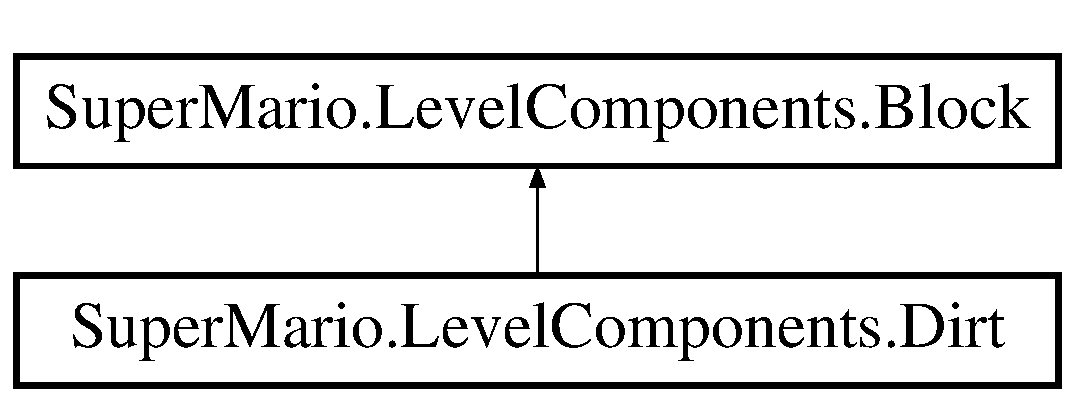
\includegraphics[height=2.000000cm]{class_super_mario_1_1_level_components_1_1_dirt}
\end{center}
\end{figure}
\subsection*{Public Member Functions}
\begin{DoxyCompactItemize}
\item 
override void \mbox{\hyperlink{class_super_mario_1_1_level_components_1_1_dirt_a800acb34aa293bf29cd3e4af39020633}{On\+Initialize}} ()
\begin{DoxyCompactList}\small\item\em This method is used to specify particular properties of the block (e.\+g. Id, Solid...) \end{DoxyCompactList}\end{DoxyCompactItemize}
\subsection*{Additional Inherited Members}


\subsection{Member Function Documentation}
\mbox{\Hypertarget{class_super_mario_1_1_level_components_1_1_dirt_a800acb34aa293bf29cd3e4af39020633}\label{class_super_mario_1_1_level_components_1_1_dirt_a800acb34aa293bf29cd3e4af39020633}} 
\index{Super\+Mario\+::\+Level\+Components\+::\+Dirt@{Super\+Mario\+::\+Level\+Components\+::\+Dirt}!On\+Initialize@{On\+Initialize}}
\index{On\+Initialize@{On\+Initialize}!Super\+Mario\+::\+Level\+Components\+::\+Dirt@{Super\+Mario\+::\+Level\+Components\+::\+Dirt}}
\subsubsection{\texorpdfstring{On\+Initialize()}{OnInitialize()}}
{\footnotesize\ttfamily override void Super\+Mario.\+Level\+Components.\+Dirt.\+On\+Initialize (\begin{DoxyParamCaption}{ }\end{DoxyParamCaption})\hspace{0.3cm}{\ttfamily [virtual]}}



This method is used to specify particular properties of the block (e.\+g. Id, Solid...) 



Implements \mbox{\hyperlink{class_super_mario_1_1_level_components_1_1_block_aecd2a6fa80ecbd7dd5cec2cdf4b149ec}{Super\+Mario.\+Level\+Components.\+Block}}.



The documentation for this class was generated from the following file\+:\begin{DoxyCompactItemize}
\item 
Level\+Components/Block.\+cs\end{DoxyCompactItemize}

\hypertarget{class_super_mario_1_1_level}{}\section{Super\+Mario.\+Level Class Reference}
\label{class_super_mario_1_1_level}\index{Super\+Mario.\+Level@{Super\+Mario.\+Level}}


The documentation for this class was generated from the following file\+:\begin{DoxyCompactItemize}
\item 
Level.\+cs\end{DoxyCompactItemize}

\hypertarget{class_super_mario_1_1_graphics_1_1_mario_small_sprite_dictionary}{}\section{Super\+Mario.\+Graphics.\+Mario\+Small\+Sprite\+Dictionary Class Reference}
\label{class_super_mario_1_1_graphics_1_1_mario_small_sprite_dictionary}\index{Super\+Mario.\+Graphics.\+Mario\+Small\+Sprite\+Dictionary@{Super\+Mario.\+Graphics.\+Mario\+Small\+Sprite\+Dictionary}}
Inheritance diagram for Super\+Mario.\+Graphics.\+Mario\+Small\+Sprite\+Dictionary\+:\begin{figure}[H]
\begin{center}
\leavevmode
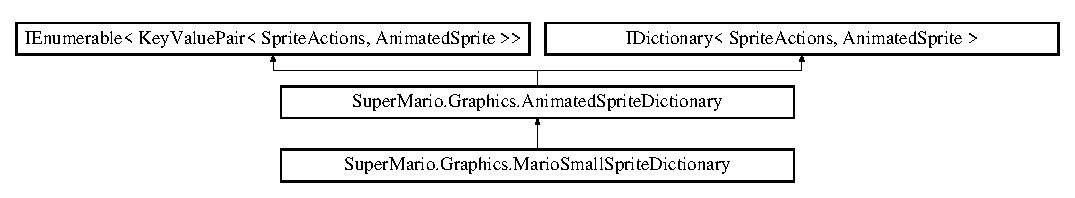
\includegraphics[height=2.210526cm]{class_super_mario_1_1_graphics_1_1_mario_small_sprite_dictionary}
\end{center}
\end{figure}
\subsection*{Protected Member Functions}
\begin{DoxyCompactItemize}
\item 
\mbox{\Hypertarget{class_super_mario_1_1_graphics_1_1_mario_small_sprite_dictionary_acc340d425eed2abfde2ef799866aa68d}\label{class_super_mario_1_1_graphics_1_1_mario_small_sprite_dictionary_acc340d425eed2abfde2ef799866aa68d}} 
override void {\bfseries Add\+Animated\+Sprites} ()
\end{DoxyCompactItemize}
\subsection*{Additional Inherited Members}


The documentation for this class was generated from the following file\+:\begin{DoxyCompactItemize}
\item 
Graphics/Animated\+Sprite\+Collection.\+cs\end{DoxyCompactItemize}

\hypertarget{class_super_mario_1_1_super_mario}{}\section{Super\+Mario.\+Super\+Mario Class Reference}
\label{class_super_mario_1_1_super_mario}\index{Super\+Mario.\+Super\+Mario@{Super\+Mario.\+Super\+Mario}}


This is the main type for your game.  


Inheritance diagram for Super\+Mario.\+Super\+Mario\+:\begin{figure}[H]
\begin{center}
\leavevmode
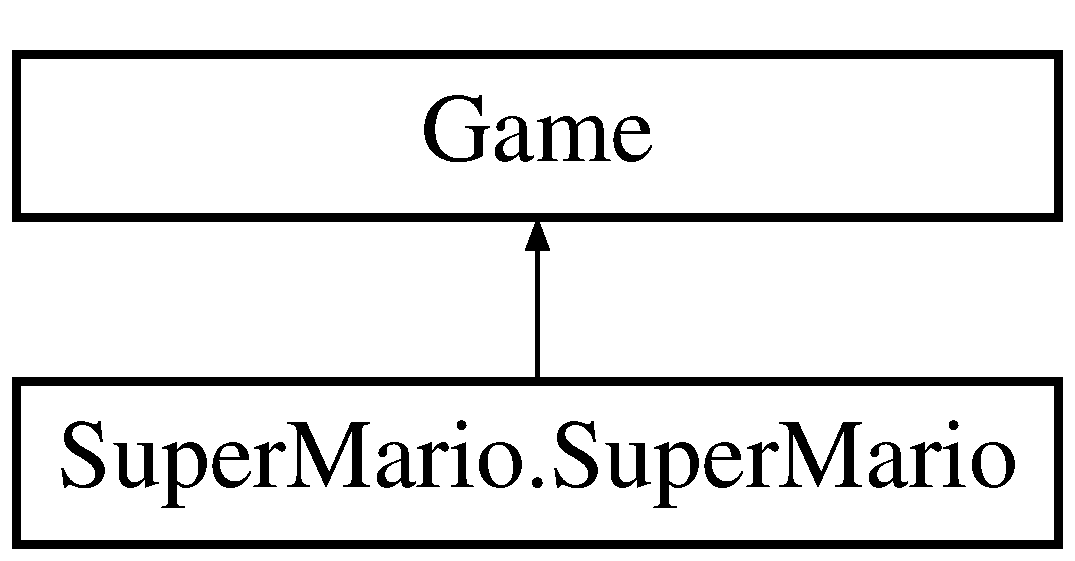
\includegraphics[height=2.000000cm]{class_super_mario_1_1_super_mario}
\end{center}
\end{figure}
\subsection*{Public Member Functions}
\begin{DoxyCompactItemize}
\item 
\mbox{\hyperlink{class_super_mario_1_1_super_mario_aaa56875411697b4bc007ec0b0c84a211}{Super\+Mario}} ()
\begin{DoxyCompactList}\small\item\em Initialize and start the game \end{DoxyCompactList}\end{DoxyCompactItemize}
\subsection*{Public Attributes}
\begin{DoxyCompactItemize}
\item 
\mbox{\hyperlink{class_super_mario_1_1_tile}{Tile}} \mbox{[},\mbox{]} \mbox{\hyperlink{class_super_mario_1_1_super_mario_a6f0b4c9d00e636d974465ea28e7b32c3}{tiles}}
\begin{DoxyCompactList}\small\item\em The level grid containing tiles infos \end{DoxyCompactList}\end{DoxyCompactItemize}
\subsection*{Protected Member Functions}
\begin{DoxyCompactItemize}
\item 
override void \mbox{\hyperlink{class_super_mario_1_1_super_mario_aa2a4ad87d65a4a7a6953eb2dce254734}{Initialize}} ()
\begin{DoxyCompactList}\small\item\em Allows the game to perform any initialization it needs to before starting to run. This is where it can query for any required services and load any non-\/graphic related content. Calling base.\+Initialize will enumerate through any components and initialize them as well. \end{DoxyCompactList}\item 
override void \mbox{\hyperlink{class_super_mario_1_1_super_mario_a5253ed5bc61d970892c4b9359de52d1e}{Load\+Content}} ()
\begin{DoxyCompactList}\small\item\em Load\+Content will be called once per game and is the place to load all of your content. \end{DoxyCompactList}\item 
override void \mbox{\hyperlink{class_super_mario_1_1_super_mario_afbf7a1973bf71e92c27161619b7af783}{Unload\+Content}} ()
\begin{DoxyCompactList}\small\item\em Unload\+Content will be called once per game and is the place to unload game-\/specific content. \end{DoxyCompactList}\item 
override void \mbox{\hyperlink{class_super_mario_1_1_super_mario_a6a180f8c2906720694ca231dfff6c4b1}{Update}} (Game\+Time game\+Time)
\begin{DoxyCompactList}\small\item\em Allows the game to run logic such as updating the world, checking for collisions, gathering input, and playing audio. \end{DoxyCompactList}\item 
override void \mbox{\hyperlink{class_super_mario_1_1_super_mario_a456a3818b9edc077d202e582cf86ac03}{Draw}} (Game\+Time game\+Time)
\begin{DoxyCompactList}\small\item\em This is called when the game should draw itself. \end{DoxyCompactList}\end{DoxyCompactItemize}
\subsection*{Properties}
\begin{DoxyCompactItemize}
\item 
static \mbox{\hyperlink{class_super_mario_1_1_super_mario}{Super\+Mario}} \mbox{\hyperlink{class_super_mario_1_1_super_mario_abac25334ac6abafdedbf46774e6a198e}{Main}}\hspace{0.3cm}{\ttfamily  \mbox{[}get\mbox{]}}
\begin{DoxyCompactList}\small\item\em Singleton instance of the game \end{DoxyCompactList}\end{DoxyCompactItemize}


\subsection{Detailed Description}
This is the main type for your game. 



\subsection{Constructor \& Destructor Documentation}
\mbox{\Hypertarget{class_super_mario_1_1_super_mario_aaa56875411697b4bc007ec0b0c84a211}\label{class_super_mario_1_1_super_mario_aaa56875411697b4bc007ec0b0c84a211}} 
\index{Super\+Mario\+::\+Super\+Mario@{Super\+Mario\+::\+Super\+Mario}!Super\+Mario@{Super\+Mario}}
\index{Super\+Mario@{Super\+Mario}!Super\+Mario\+::\+Super\+Mario@{Super\+Mario\+::\+Super\+Mario}}
\subsubsection{\texorpdfstring{Super\+Mario()}{SuperMario()}}
{\footnotesize\ttfamily Super\+Mario.\+Super\+Mario.\+Super\+Mario (\begin{DoxyParamCaption}{ }\end{DoxyParamCaption})}



Initialize and start the game 



\subsection{Member Function Documentation}
\mbox{\Hypertarget{class_super_mario_1_1_super_mario_a456a3818b9edc077d202e582cf86ac03}\label{class_super_mario_1_1_super_mario_a456a3818b9edc077d202e582cf86ac03}} 
\index{Super\+Mario\+::\+Super\+Mario@{Super\+Mario\+::\+Super\+Mario}!Draw@{Draw}}
\index{Draw@{Draw}!Super\+Mario\+::\+Super\+Mario@{Super\+Mario\+::\+Super\+Mario}}
\subsubsection{\texorpdfstring{Draw()}{Draw()}}
{\footnotesize\ttfamily override void Super\+Mario.\+Super\+Mario.\+Draw (\begin{DoxyParamCaption}\item[{Game\+Time}]{game\+Time }\end{DoxyParamCaption})\hspace{0.3cm}{\ttfamily [protected]}}



This is called when the game should draw itself. 


\begin{DoxyParams}{Parameters}
{\em game\+Time} & Provides a snapshot of timing values.\\
\hline
\end{DoxyParams}
\mbox{\Hypertarget{class_super_mario_1_1_super_mario_aa2a4ad87d65a4a7a6953eb2dce254734}\label{class_super_mario_1_1_super_mario_aa2a4ad87d65a4a7a6953eb2dce254734}} 
\index{Super\+Mario\+::\+Super\+Mario@{Super\+Mario\+::\+Super\+Mario}!Initialize@{Initialize}}
\index{Initialize@{Initialize}!Super\+Mario\+::\+Super\+Mario@{Super\+Mario\+::\+Super\+Mario}}
\subsubsection{\texorpdfstring{Initialize()}{Initialize()}}
{\footnotesize\ttfamily override void Super\+Mario.\+Super\+Mario.\+Initialize (\begin{DoxyParamCaption}{ }\end{DoxyParamCaption})\hspace{0.3cm}{\ttfamily [protected]}}



Allows the game to perform any initialization it needs to before starting to run. This is where it can query for any required services and load any non-\/graphic related content. Calling base.\+Initialize will enumerate through any components and initialize them as well. 

\mbox{\Hypertarget{class_super_mario_1_1_super_mario_a5253ed5bc61d970892c4b9359de52d1e}\label{class_super_mario_1_1_super_mario_a5253ed5bc61d970892c4b9359de52d1e}} 
\index{Super\+Mario\+::\+Super\+Mario@{Super\+Mario\+::\+Super\+Mario}!Load\+Content@{Load\+Content}}
\index{Load\+Content@{Load\+Content}!Super\+Mario\+::\+Super\+Mario@{Super\+Mario\+::\+Super\+Mario}}
\subsubsection{\texorpdfstring{Load\+Content()}{LoadContent()}}
{\footnotesize\ttfamily override void Super\+Mario.\+Super\+Mario.\+Load\+Content (\begin{DoxyParamCaption}{ }\end{DoxyParamCaption})\hspace{0.3cm}{\ttfamily [protected]}}



Load\+Content will be called once per game and is the place to load all of your content. 

\mbox{\Hypertarget{class_super_mario_1_1_super_mario_afbf7a1973bf71e92c27161619b7af783}\label{class_super_mario_1_1_super_mario_afbf7a1973bf71e92c27161619b7af783}} 
\index{Super\+Mario\+::\+Super\+Mario@{Super\+Mario\+::\+Super\+Mario}!Unload\+Content@{Unload\+Content}}
\index{Unload\+Content@{Unload\+Content}!Super\+Mario\+::\+Super\+Mario@{Super\+Mario\+::\+Super\+Mario}}
\subsubsection{\texorpdfstring{Unload\+Content()}{UnloadContent()}}
{\footnotesize\ttfamily override void Super\+Mario.\+Super\+Mario.\+Unload\+Content (\begin{DoxyParamCaption}{ }\end{DoxyParamCaption})\hspace{0.3cm}{\ttfamily [protected]}}



Unload\+Content will be called once per game and is the place to unload game-\/specific content. 

\mbox{\Hypertarget{class_super_mario_1_1_super_mario_a6a180f8c2906720694ca231dfff6c4b1}\label{class_super_mario_1_1_super_mario_a6a180f8c2906720694ca231dfff6c4b1}} 
\index{Super\+Mario\+::\+Super\+Mario@{Super\+Mario\+::\+Super\+Mario}!Update@{Update}}
\index{Update@{Update}!Super\+Mario\+::\+Super\+Mario@{Super\+Mario\+::\+Super\+Mario}}
\subsubsection{\texorpdfstring{Update()}{Update()}}
{\footnotesize\ttfamily override void Super\+Mario.\+Super\+Mario.\+Update (\begin{DoxyParamCaption}\item[{Game\+Time}]{game\+Time }\end{DoxyParamCaption})\hspace{0.3cm}{\ttfamily [protected]}}



Allows the game to run logic such as updating the world, checking for collisions, gathering input, and playing audio. 


\begin{DoxyParams}{Parameters}
{\em game\+Time} & Provides a snapshot of timing values.\\
\hline
\end{DoxyParams}


\subsection{Member Data Documentation}
\mbox{\Hypertarget{class_super_mario_1_1_super_mario_a6f0b4c9d00e636d974465ea28e7b32c3}\label{class_super_mario_1_1_super_mario_a6f0b4c9d00e636d974465ea28e7b32c3}} 
\index{Super\+Mario\+::\+Super\+Mario@{Super\+Mario\+::\+Super\+Mario}!tiles@{tiles}}
\index{tiles@{tiles}!Super\+Mario\+::\+Super\+Mario@{Super\+Mario\+::\+Super\+Mario}}
\subsubsection{\texorpdfstring{tiles}{tiles}}
{\footnotesize\ttfamily \mbox{\hyperlink{class_super_mario_1_1_tile}{Tile}} \mbox{[},\mbox{]} Super\+Mario.\+Super\+Mario.\+tiles}



The level grid containing tiles infos 



\subsection{Property Documentation}
\mbox{\Hypertarget{class_super_mario_1_1_super_mario_abac25334ac6abafdedbf46774e6a198e}\label{class_super_mario_1_1_super_mario_abac25334ac6abafdedbf46774e6a198e}} 
\index{Super\+Mario\+::\+Super\+Mario@{Super\+Mario\+::\+Super\+Mario}!Main@{Main}}
\index{Main@{Main}!Super\+Mario\+::\+Super\+Mario@{Super\+Mario\+::\+Super\+Mario}}
\subsubsection{\texorpdfstring{Main}{Main}}
{\footnotesize\ttfamily \mbox{\hyperlink{class_super_mario_1_1_super_mario}{Super\+Mario}} Super\+Mario.\+Super\+Mario.\+Main\hspace{0.3cm}{\ttfamily [static]}, {\ttfamily [get]}}



Singleton instance of the game 



The documentation for this class was generated from the following file\+:\begin{DoxyCompactItemize}
\item 
Super\+Mario.\+cs\end{DoxyCompactItemize}

\hypertarget{class_super_mario_1_1_tile}{}\section{Super\+Mario.\+Tile Class Reference}
\label{class_super_mario_1_1_tile}\index{Super\+Mario.\+Tile@{Super\+Mario.\+Tile}}


Class that store infos about a particular tile  


\subsection*{Public Member Functions}
\begin{DoxyCompactItemize}
\item 
\mbox{\hyperlink{class_super_mario_1_1_tile_a564fe1be7202cb3f3aadb75d38e6b993}{Tile}} ()
\begin{DoxyCompactList}\small\item\em Default constructor used to initialize the main array with empty tiles \end{DoxyCompactList}\item 
\mbox{\hyperlink{class_super_mario_1_1_tile_a27450d36e4f8d7aa7bb8737eebd9aea8}{Tile}} (int block\+Id, int wall\+Id)
\begin{DoxyCompactList}\small\item\em Constructor to set a non-\/default tile \end{DoxyCompactList}\end{DoxyCompactItemize}
\subsection*{Public Attributes}
\begin{DoxyCompactItemize}
\item 
int \mbox{\hyperlink{class_super_mario_1_1_tile_a2568c2548122e42a75208f2a3bc851fe}{Wall\+Id}}
\begin{DoxyCompactList}\small\item\em The id of the background object, used as key to access the access the walls Dictionary. Set to -\/1 to set as empty \end{DoxyCompactList}\item 
bool \mbox{\hyperlink{class_super_mario_1_1_tile_a870427fd1ed65b69ae920c863bd46a2c}{Solid}} = true
\begin{DoxyCompactList}\small\item\em Determines whether the player can pass through it \end{DoxyCompactList}\item 
bool \mbox{\hyperlink{class_super_mario_1_1_tile_a033ea68f20db786cf3f71d9b3351e523}{Platform}}
\begin{DoxyCompactList}\small\item\em Determines if the block should behave as a platform \end{DoxyCompactList}\end{DoxyCompactItemize}
\subsection*{Properties}
\begin{DoxyCompactItemize}
\item 
int \mbox{\hyperlink{class_super_mario_1_1_tile_a2bbfc4d23dcecaf5e3c1fee0501fae55}{Block\+Id}}\hspace{0.3cm}{\ttfamily  \mbox{[}get, set\mbox{]}}
\begin{DoxyCompactList}\small\item\em The id of the foreground object, used as key to access the access the blocks Dictionary. Set to -\/1 to set as empty \end{DoxyCompactList}\end{DoxyCompactItemize}


\subsection{Detailed Description}
Class that store infos about a particular tile 



\subsection{Constructor \& Destructor Documentation}
\mbox{\Hypertarget{class_super_mario_1_1_tile_a564fe1be7202cb3f3aadb75d38e6b993}\label{class_super_mario_1_1_tile_a564fe1be7202cb3f3aadb75d38e6b993}} 
\index{Super\+Mario\+::\+Tile@{Super\+Mario\+::\+Tile}!Tile@{Tile}}
\index{Tile@{Tile}!Super\+Mario\+::\+Tile@{Super\+Mario\+::\+Tile}}
\subsubsection{\texorpdfstring{Tile()}{Tile()}\hspace{0.1cm}{\footnotesize\ttfamily [1/2]}}
{\footnotesize\ttfamily Super\+Mario.\+Tile.\+Tile (\begin{DoxyParamCaption}{ }\end{DoxyParamCaption})}



Default constructor used to initialize the main array with empty tiles 

\mbox{\Hypertarget{class_super_mario_1_1_tile_a27450d36e4f8d7aa7bb8737eebd9aea8}\label{class_super_mario_1_1_tile_a27450d36e4f8d7aa7bb8737eebd9aea8}} 
\index{Super\+Mario\+::\+Tile@{Super\+Mario\+::\+Tile}!Tile@{Tile}}
\index{Tile@{Tile}!Super\+Mario\+::\+Tile@{Super\+Mario\+::\+Tile}}
\subsubsection{\texorpdfstring{Tile()}{Tile()}\hspace{0.1cm}{\footnotesize\ttfamily [2/2]}}
{\footnotesize\ttfamily Super\+Mario.\+Tile.\+Tile (\begin{DoxyParamCaption}\item[{int}]{block\+Id,  }\item[{int}]{wall\+Id }\end{DoxyParamCaption})}



Constructor to set a non-\/default tile 


\begin{DoxyParams}{Parameters}
{\em block\+Id} & The Id of the \mbox{\hyperlink{class_super_mario_1_1_level_components_1_1_block}{Level\+Components.\+Block}}\\
\hline
{\em wall\+Id} & The id of the \mbox{\hyperlink{class_super_mario_1_1_level_components_1_1_wall}{Level\+Components.\+Wall}}\\
\hline
\end{DoxyParams}


\subsection{Member Data Documentation}
\mbox{\Hypertarget{class_super_mario_1_1_tile_a033ea68f20db786cf3f71d9b3351e523}\label{class_super_mario_1_1_tile_a033ea68f20db786cf3f71d9b3351e523}} 
\index{Super\+Mario\+::\+Tile@{Super\+Mario\+::\+Tile}!Platform@{Platform}}
\index{Platform@{Platform}!Super\+Mario\+::\+Tile@{Super\+Mario\+::\+Tile}}
\subsubsection{\texorpdfstring{Platform}{Platform}}
{\footnotesize\ttfamily bool Super\+Mario.\+Tile.\+Platform}



Determines if the block should behave as a platform 

\mbox{\Hypertarget{class_super_mario_1_1_tile_a870427fd1ed65b69ae920c863bd46a2c}\label{class_super_mario_1_1_tile_a870427fd1ed65b69ae920c863bd46a2c}} 
\index{Super\+Mario\+::\+Tile@{Super\+Mario\+::\+Tile}!Solid@{Solid}}
\index{Solid@{Solid}!Super\+Mario\+::\+Tile@{Super\+Mario\+::\+Tile}}
\subsubsection{\texorpdfstring{Solid}{Solid}}
{\footnotesize\ttfamily bool Super\+Mario.\+Tile.\+Solid = true}



Determines whether the player can pass through it 

\mbox{\Hypertarget{class_super_mario_1_1_tile_a2568c2548122e42a75208f2a3bc851fe}\label{class_super_mario_1_1_tile_a2568c2548122e42a75208f2a3bc851fe}} 
\index{Super\+Mario\+::\+Tile@{Super\+Mario\+::\+Tile}!Wall\+Id@{Wall\+Id}}
\index{Wall\+Id@{Wall\+Id}!Super\+Mario\+::\+Tile@{Super\+Mario\+::\+Tile}}
\subsubsection{\texorpdfstring{Wall\+Id}{WallId}}
{\footnotesize\ttfamily int Super\+Mario.\+Tile.\+Wall\+Id}



The id of the background object, used as key to access the access the walls Dictionary. Set to -\/1 to set as empty 



\subsection{Property Documentation}
\mbox{\Hypertarget{class_super_mario_1_1_tile_a2bbfc4d23dcecaf5e3c1fee0501fae55}\label{class_super_mario_1_1_tile_a2bbfc4d23dcecaf5e3c1fee0501fae55}} 
\index{Super\+Mario\+::\+Tile@{Super\+Mario\+::\+Tile}!Block\+Id@{Block\+Id}}
\index{Block\+Id@{Block\+Id}!Super\+Mario\+::\+Tile@{Super\+Mario\+::\+Tile}}
\subsubsection{\texorpdfstring{Block\+Id}{BlockId}}
{\footnotesize\ttfamily int Super\+Mario.\+Tile.\+Block\+Id\hspace{0.3cm}{\ttfamily [get]}, {\ttfamily [set]}}



The id of the foreground object, used as key to access the access the blocks Dictionary. Set to -\/1 to set as empty 



The documentation for this class was generated from the following file\+:\begin{DoxyCompactItemize}
\item 
Tile.\+cs\end{DoxyCompactItemize}

\hypertarget{class_super_mario_1_1_level_components_1_1_wall}{}\section{Super\+Mario.\+Level\+Components.\+Wall Class Reference}
\label{class_super_mario_1_1_level_components_1_1_wall}\index{Super\+Mario.\+Level\+Components.\+Wall@{Super\+Mario.\+Level\+Components.\+Wall}}


This class contains all the data for background objects  


\subsection*{Public Member Functions}
\begin{DoxyCompactItemize}
\item 
\mbox{\hyperlink{class_super_mario_1_1_level_components_1_1_wall_a8289646ed2e3bab70d6ed13144997318}{Wall}} ()
\begin{DoxyCompactList}\small\item\em T\+O\+DO constructor \end{DoxyCompactList}\end{DoxyCompactItemize}
\subsection*{Public Attributes}
\begin{DoxyCompactItemize}
\item 
readonly Texture2D \mbox{\hyperlink{class_super_mario_1_1_level_components_1_1_wall_a336f1410914c4832d5db575a8540183b}{tile\+Set}}
\begin{DoxyCompactList}\small\item\em The texture Atlas \end{DoxyCompactList}\end{DoxyCompactItemize}


\subsection{Detailed Description}
This class contains all the data for background objects 



\subsection{Constructor \& Destructor Documentation}
\mbox{\Hypertarget{class_super_mario_1_1_level_components_1_1_wall_a8289646ed2e3bab70d6ed13144997318}\label{class_super_mario_1_1_level_components_1_1_wall_a8289646ed2e3bab70d6ed13144997318}} 
\index{Super\+Mario\+::\+Level\+Components\+::\+Wall@{Super\+Mario\+::\+Level\+Components\+::\+Wall}!Wall@{Wall}}
\index{Wall@{Wall}!Super\+Mario\+::\+Level\+Components\+::\+Wall@{Super\+Mario\+::\+Level\+Components\+::\+Wall}}
\subsubsection{\texorpdfstring{Wall()}{Wall()}}
{\footnotesize\ttfamily Super\+Mario.\+Level\+Components.\+Wall.\+Wall (\begin{DoxyParamCaption}{ }\end{DoxyParamCaption})}



T\+O\+DO constructor 



\subsection{Member Data Documentation}
\mbox{\Hypertarget{class_super_mario_1_1_level_components_1_1_wall_a336f1410914c4832d5db575a8540183b}\label{class_super_mario_1_1_level_components_1_1_wall_a336f1410914c4832d5db575a8540183b}} 
\index{Super\+Mario\+::\+Level\+Components\+::\+Wall@{Super\+Mario\+::\+Level\+Components\+::\+Wall}!tile\+Set@{tile\+Set}}
\index{tile\+Set@{tile\+Set}!Super\+Mario\+::\+Level\+Components\+::\+Wall@{Super\+Mario\+::\+Level\+Components\+::\+Wall}}
\subsubsection{\texorpdfstring{tile\+Set}{tileSet}}
{\footnotesize\ttfamily readonly Texture2D Super\+Mario.\+Level\+Components.\+Wall.\+tile\+Set}



The texture Atlas 



The documentation for this class was generated from the following file\+:\begin{DoxyCompactItemize}
\item 
Level\+Components/Wall.\+cs\end{DoxyCompactItemize}

%--- End generated contents ---

% Index
\backmatter
\newpage
\phantomsection
\clearemptydoublepage
\addcontentsline{toc}{chapter}{Index}
\printindex

\end{document}
